\documentclass{ximera}

\typeout{Start loading xmPreamble.tex}%

% Add here extra macro's that are loaded automatically by all documents of claas 'ximera' or 'xourse' in this repo

%%
%%  Example:
%%
% \newcommand{\R}{\mathbb{R}

\title{Lesson 1: Making Calculations (And Getting to Know the Layout)}
\begin{document}

\begin{abstract}
In this lesson, we will explore basic calculations and how to work with variables in MATLAB.
\end{abstract}

\section*{Activity 1: Getting to Know MATLAB}

In this activity, we'll cover basic calculations and how to work with variables in MATLAB. 
First, let's take a look at the setup of MATLAB. Feel free to reference these images as needed.

\subsection*{MATLAB Online Setup}

If you're using MATLAB Online, after opening up a live script your setup should look something like this:

\begin{center}
    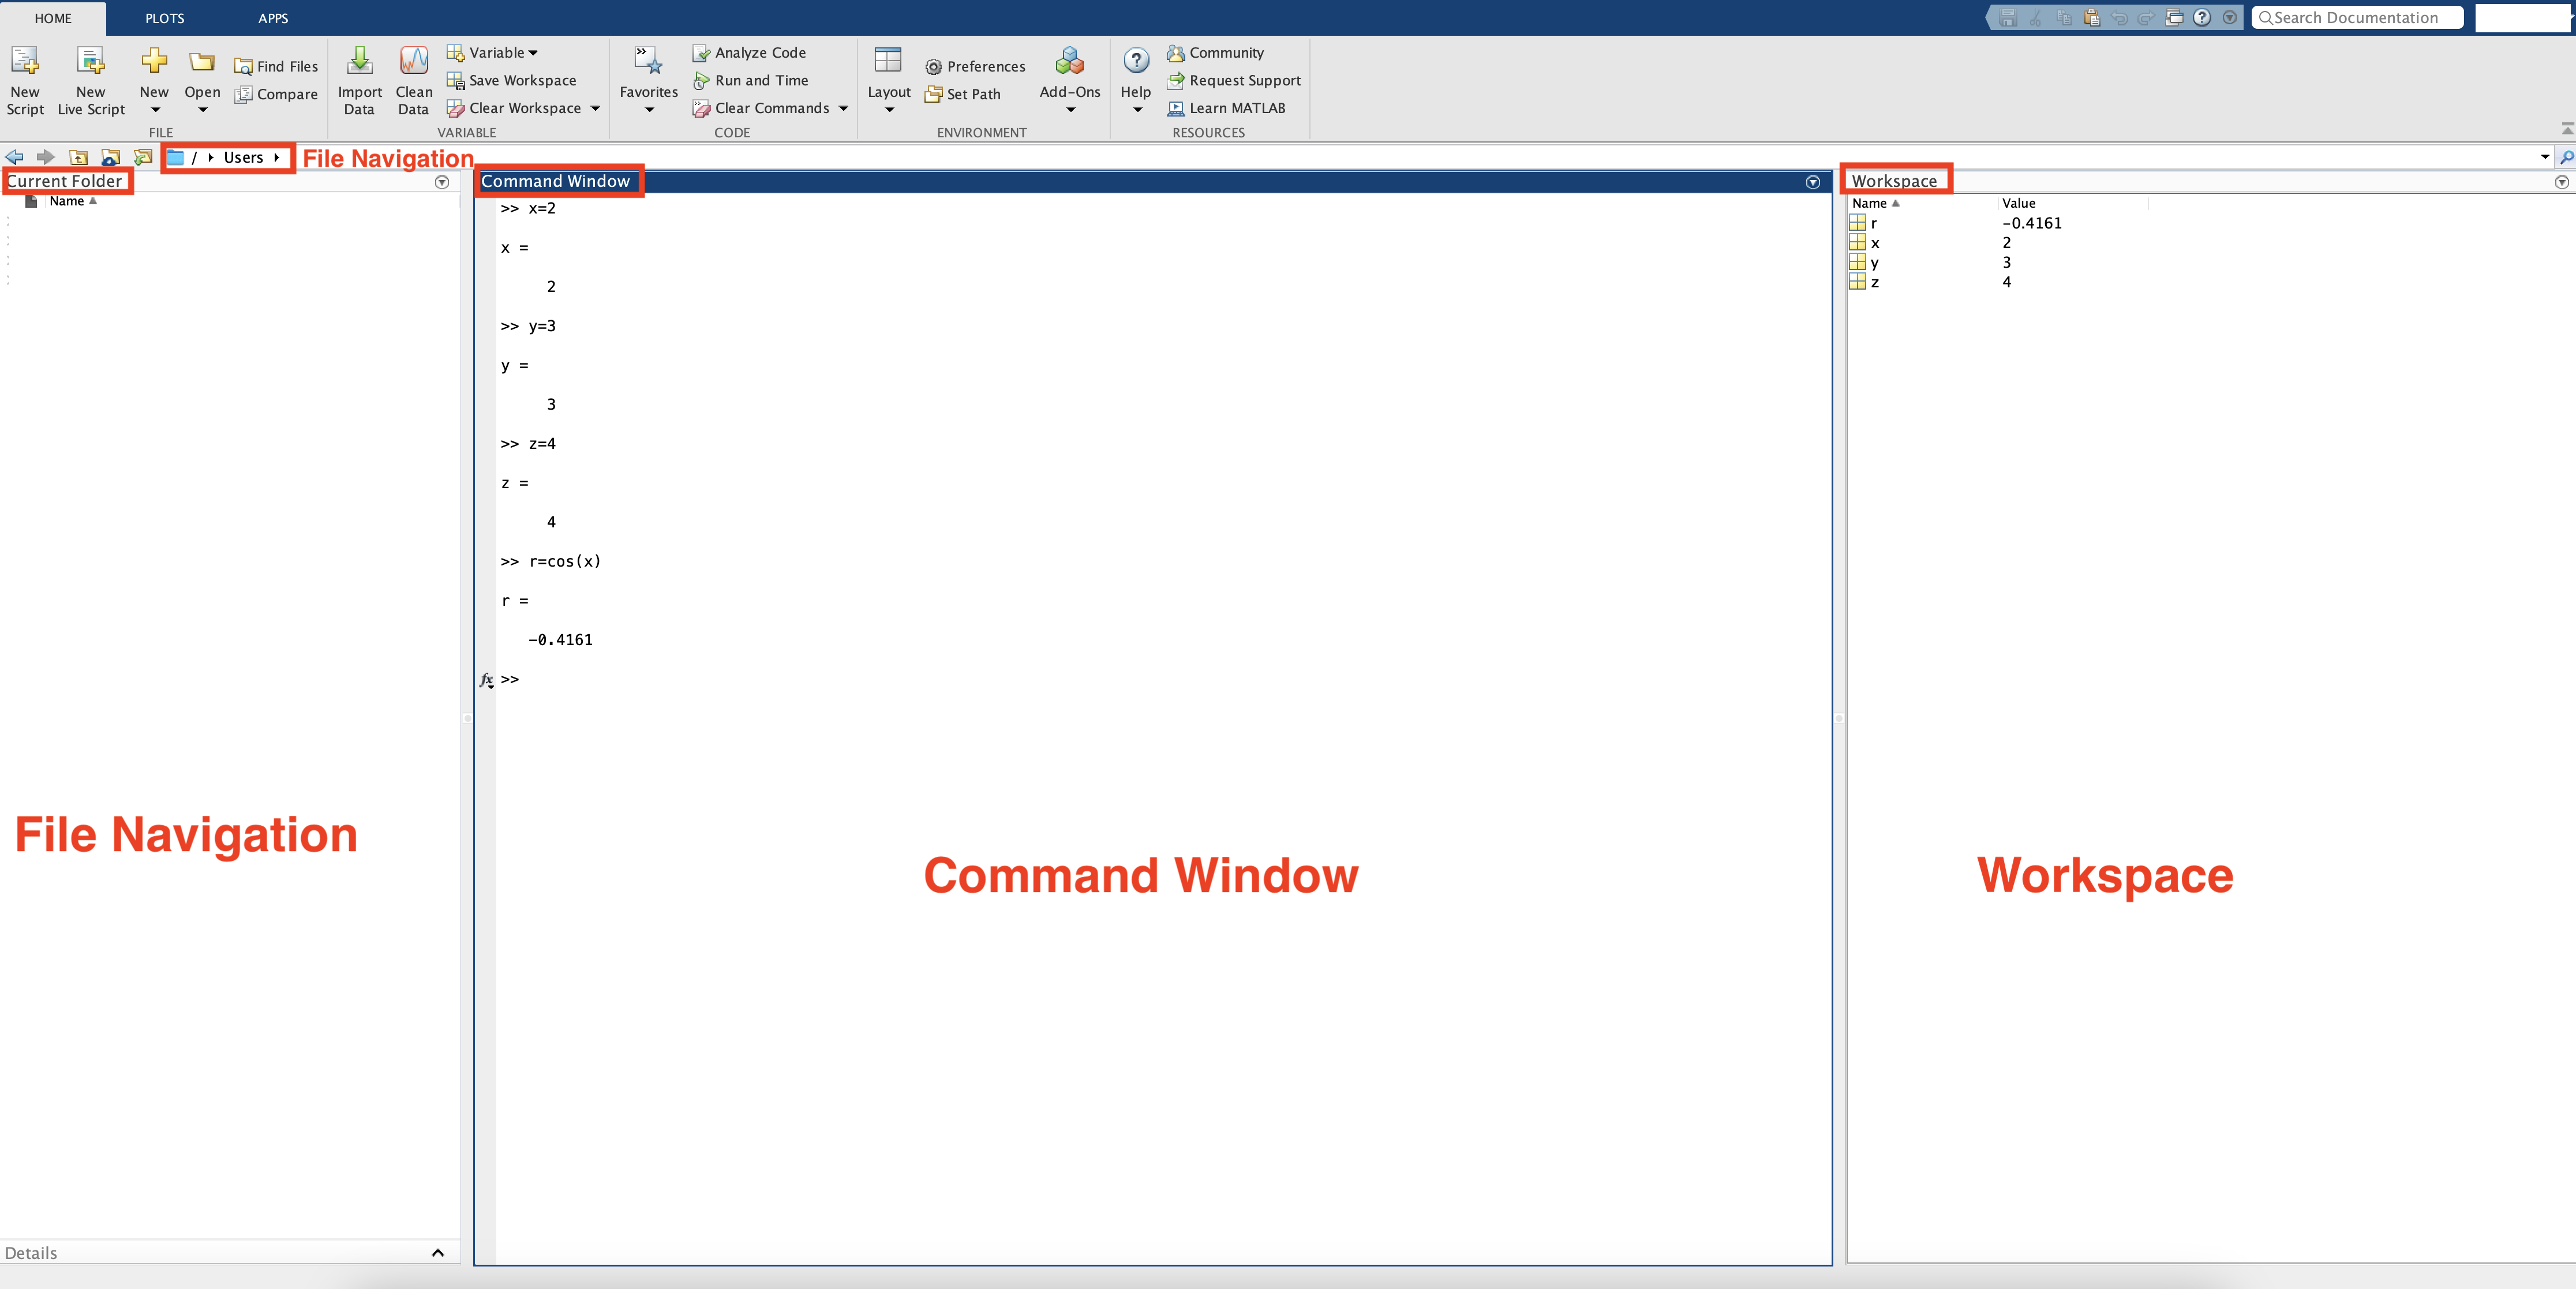
\includegraphics[width=0.8\textwidth]{MATLAB_Home_Screen.png}
\end{center}

\subsection*{MATLAB Downloaded Setup}

Within a live script, the interface will appear as follows. This window is separate from the command window and workspace.

% \begin{center}
% \includegraphics[width=0.8\textwidth]{matlab_downloaded_setup.png}
% \end{center}

The workspace and command window appear as follows:

% \begin{center}
% \includegraphics[width=0.8\textwidth]{matlab_workspace.png}
% \end{center}

\section*{Activity 2: Basic Calculations and Variables}

Let's start by performing some basic math operations. Suppose you're driving a car and travel 100 meters in 20 seconds.
In the code below, type out the calculation that determines the speed of the car in meters per second.

\textbf{Note:} MATLAB ignores anything after a \texttt{\%} sign. This is called a \textbf{comment}, and you can use it to add notes. 
Comments can be placed on the same line as the code, and anything before \texttt{\%} is executed while anything after is ignored.

\begin{verbatim}
% Use the "/" sign to divide 100 meters by 20 seconds
100 / 20
\end{verbatim}

This operation is similar to what you might enter in a graphing calculator.

To execute this command, select the \textbf{"Run Section"} button in the live script. MATLAB will run this computation, 
and the answer will appear on the right side of the screen labeled as \texttt{ans}.

\textbf{Note:} The large green \textbf{"Run"} button executes the entire live script from top to bottom, rather than just the selected section.

You should see the following output:

\begin{verbatim}
ans = 5
\end{verbatim}

(5 meters per second is approximately 11 miles per hour).

\end{document}